\chapter{Progetto di \textit{stage}}
    \section{Gestione degli \textit{stage} in SogeaSoft S.r.l.}
    SogeaSoft S.r.l. riconosce il valore strategico degli \textit{stage} curricolari, considerandoli un'opportunità sia per la formazione di potenziali nuovi dipendenti, sia per l'esplorazione di nuove tecnologie e la valutazione critica dei sistemi attualmente in uso. Tali percorsi formativi consentono non solo di trasferire conoscenze e competenze, ma anche di promuovere un'analisi approfondita delle soluzioni tecnologiche adottate dall'azienda, favorendo l'innovazione e l'ottimizzazione dei processi.  

    \vspace{0.2 em}
    \noindent Da ciò che ho potuto comprendere durante il mio periodo a SogeaSoft S.r.l., le attività svolte nell'ambito degli \textit{stage} possono includere: 
    \begin{itemize}
        \item l'integrazione di nuove funzionalità nei sistemi esistenti, con l'obiettivo di migliorarne le prestazioni e l'efficienza;
        \item lo studio e lo sviluppo di strumenti autonomi a supporto dei processi di sviluppo o dei prodotti in uso, come ad esempio Swagger, una piattaforma per la documentazione e il \textit{testing} delle API (approfondite nella Sezione 1.7);  
        \item l'analisi formale di strumenti già utilizzati in azienda, ma impiegati prevalentemente in modo empirico, al fine di standardizzarne e ottimizzarne l'uso;  
        \item la conduzione di attività di monitoraggio sulle \textit{performance} di determinati sistemi, per identificarne eventuali criticità e proporre soluzioni migliorative.  
    \end{itemize}

    \vspace{0.2 em}
    \noindent L'evoluzione tecnologica in SogeaSoft S.r.l. può avvenire attraverso diverse strategie, tra cui l'ampliamento delle funzionalità della \textit{codebase} esistente, l'analisi teorica dello stato dell'arte o la realizzazione di \textit{software} sperimentali, quali \textit{Proof of $Concept_G$} ($PoC_G$) o prodotti già pronti per un utilizzo immediato, come il \textit{Minimum Viable $Product_G$} ($MVP_G$). Nel contesto del mio \textit{stage}, le attività svolte hanno combinato questi approcci, consentendo lo sviluppo di una soluzione concreta ma non immediatamente utilizzabile (ossia un \text{prototipo\textsubscript{G}}, la cui differenza è visibile nella Figura \ref{fig:PoC-prototipo-MVP}); nonché la produzione di una documentazione tecnica approfondita.  
    
    \begin{figure}[H]
        \centering
        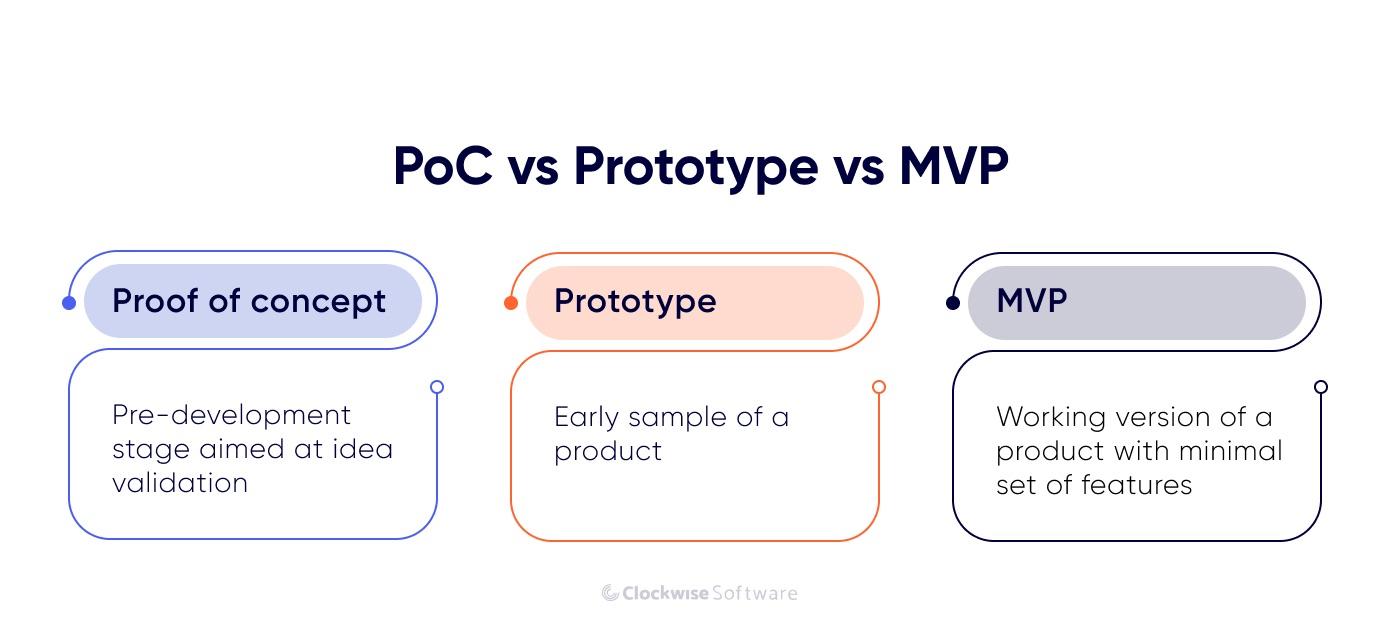
\includegraphics[width=0.6\linewidth]{BCS-Tessi/images/PoC_MVP.jpeg}
        \caption[Differenza tra PoC, Prototipo, MVP]{Differenza tra PoC, Prototipo, MVP. Fonte: https://clockwise.software/blog/proof-of-concept-in-software-development/ \textit{(ultimo accesso 12/03/2025)}}
        \label{fig:PoC-prototipo-MVP}
    \end{figure}

    \vspace{0.2 em}
    \noindent SogeaSoft S.r.l. attribuisce particolare valore agli \textit{stage}, poiché rappresentano un'opportunità strategica per affrontare una delle sue principali sfide tecnologiche: la migrazione del proprio prodotto da un'architettura $monolitica_G$ a un'architettura a $microservizi_G$, come discusso nella Sezione 1.8. Gli \textit{stage} costituiscono una risorsa vantaggiosa sotto molteplici aspetti: da un lato, permettono di ottimizzare l'investimento in ricerca e sviluppo grazie a costi contenuti; dall'altro, consentono all'azienda di entrare in contatto con prospettive innovative, idee originali e persone non condizionate da paradigmi consolidati. 

    \vspace{0.2 em}
    \noindent Un ulteriore fattore determinante nell'impiego di tirocinanti per lo sviluppo di soluzioni innovative è la gestione delle risorse interne. Il personale aziendale è prevalentemente impegnato nel mantenimento e nell'evoluzione dei sistemi attualmente in produzione, rendendo complesso il reindirizzamento delle competenze su progetti sperimentali. L'inserimento di studenti permette di destinare risorse dedicate a iniziative di ricerca e innovazione, permettendo al contempo un processo di trasferimento di conoscenze tra le diverse generazioni di sviluppatori.
    
    \section{Il \textit{software} SAIonWeb}
    
    Il tema principale del mio \textit{stage} ha riguardato lo sviluppo e l'evoluzione di SAIonWeb, un \textit{software} basato sul \textit{framework} SAI (Sistema Aziendale Integrato). SAIonWeb è uno strumento progettato per la gestione dei processi aziendali nell'ambito dell'\textit{Enterprise Resource Planning} (ERP). In particolare, il \textit{software} è stato concepito per rispondere alle esigenze specifiche del settore manifatturiero, nello specifico all'industria dell'abbigliamento, offrendo supporto integrato all'intero ciclo di vita del prodotto: dalla gestione e approvvigionamento delle materie prime, attraverso la fase di confezionamento e produzione, fino alla distribuzione e commercializzazione finale\footnote{Fonte: https://sogeasoft.com/p/sai \textit{(ultima visita 12/03/2025)}}. 

    \begin{figure}[H]
        \centering
        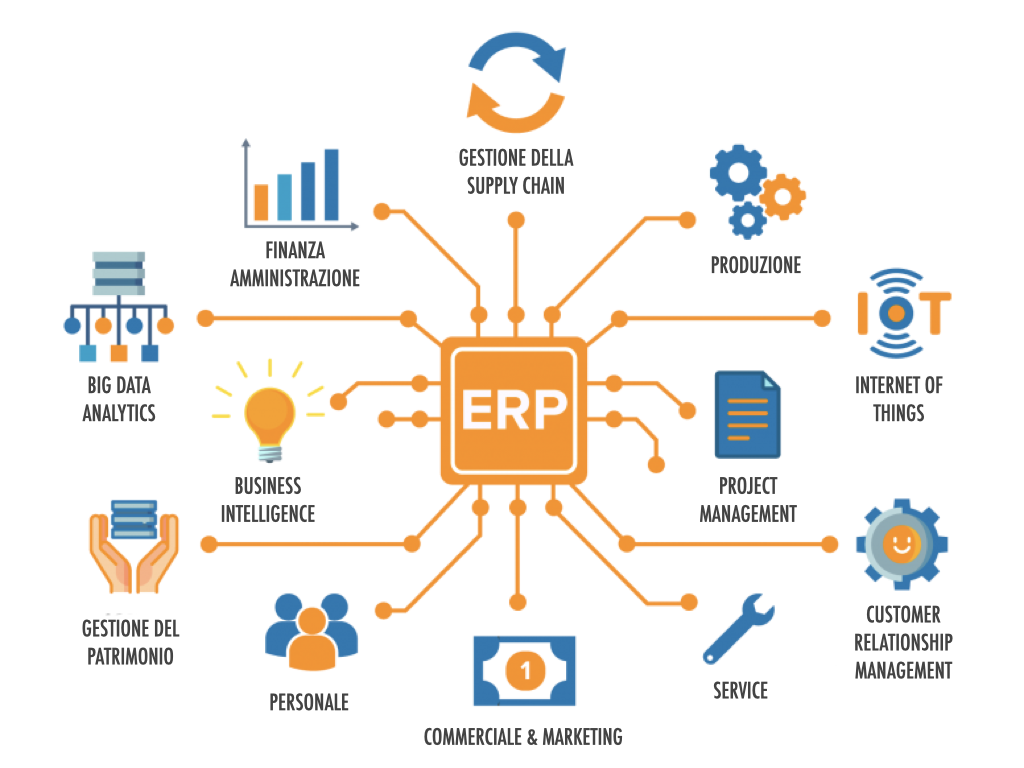
\includegraphics[width=0.5\linewidth]{BCS-Tessi//images/ERP.png}
        \caption[Esempio di un ERP generico]{Esempio di un ERP generico. Fonte:https://www.bo.camcom.gov.it/it/promozione-interna/sistemi-gestionali-erp \textit{(ultima visita 15/03/2025)}}
        \label{fig:ERP}
    \end{figure}

    \vspace{0.2 em}
    \noindent Come anticipato nella Sezione 1.2, SAIonWeb costituisce uno strumento di elevata rilevanza strategica, implementato da diverse realtà imprenditoriali operanti nel settore manifatturiero, con l'obiettivo di automatizzare e ottimizzare molteplici processi operativi aziendali. I processi specifici supportati dal sistema e le relative implicazioni funzionali sono oggetto di approfondimento nella sezione successiva.
    
        \subsection{Funzionalità generali di SAIonWeb}
        SAI ERP (e dunque anche SAIonWeb) è un sistema \textit{software} gestionale progettato per integrare e automatizzare i processi aziendali, consentendo alle organizzazioni di gestire in modo efficiente risorse, dati e operazioni. Questi sistemi offrono un ambiente centralizzato in cui le diverse aree aziendali, dalla produzione alla logistica, dalla contabilità alla gestione delle risorse umane, possono operare in modo coordinato, migliorando la tracciabilità delle informazioni e ottimizzando la produttività.  

        \vspace{0.2 em}
        \noindent Le sue funzionalità principali includono:  
        \begin{itemize}
            \item \textbf{gestione delle materie prime}: monitoraggio degli approvvigionamenti, delle scorte e della qualità dei materiali;
            \item \textbf{pianificazione della produzione}: organizzazione delle fasi produttive, assegnazione delle risorse e gestione dei tempi di lavorazione;
            \item \textbf{tracciabilità dei prodotti}: controllo dell'avanzamento di ciascun capo, dalla fase iniziale di lavorazione fino alla distribuzione. In particolare, una schermata d'esempio è visibile in Figura \ref{fig:screenSAI};
            \item \textbf{gestione degli ordini e delle vendite}: registrazione degli ordini, gestione delle consegne e fatturazione automatizzata;
            \item \textbf{logistica e distribuzione}: coordinamento delle spedizioni, gestione dei magazzini e ottimizzazione delle scorte;
            \item \textbf{integrazione con il sistema contabile}: gestione di pagamenti, bilanci e rendicontazione finanziaria;
            \item \textbf{monitoraggio delle performance aziendali}: generazione di \textit{report} analitici e strumenti di \textit{business intelligence} per supportare il processo decisionale.  
        \end{itemize}

        \vspace{0.2 em}
        \noindent Attraverso queste funzionalità, SAI e SAIonWeb consentono alle aziende del settore moda di migliorare la gestione delle operazioni, ridurre i tempi di produzione e garantire una maggiore efficienza operativa.

        \begin{figure}[H]
            \centering
            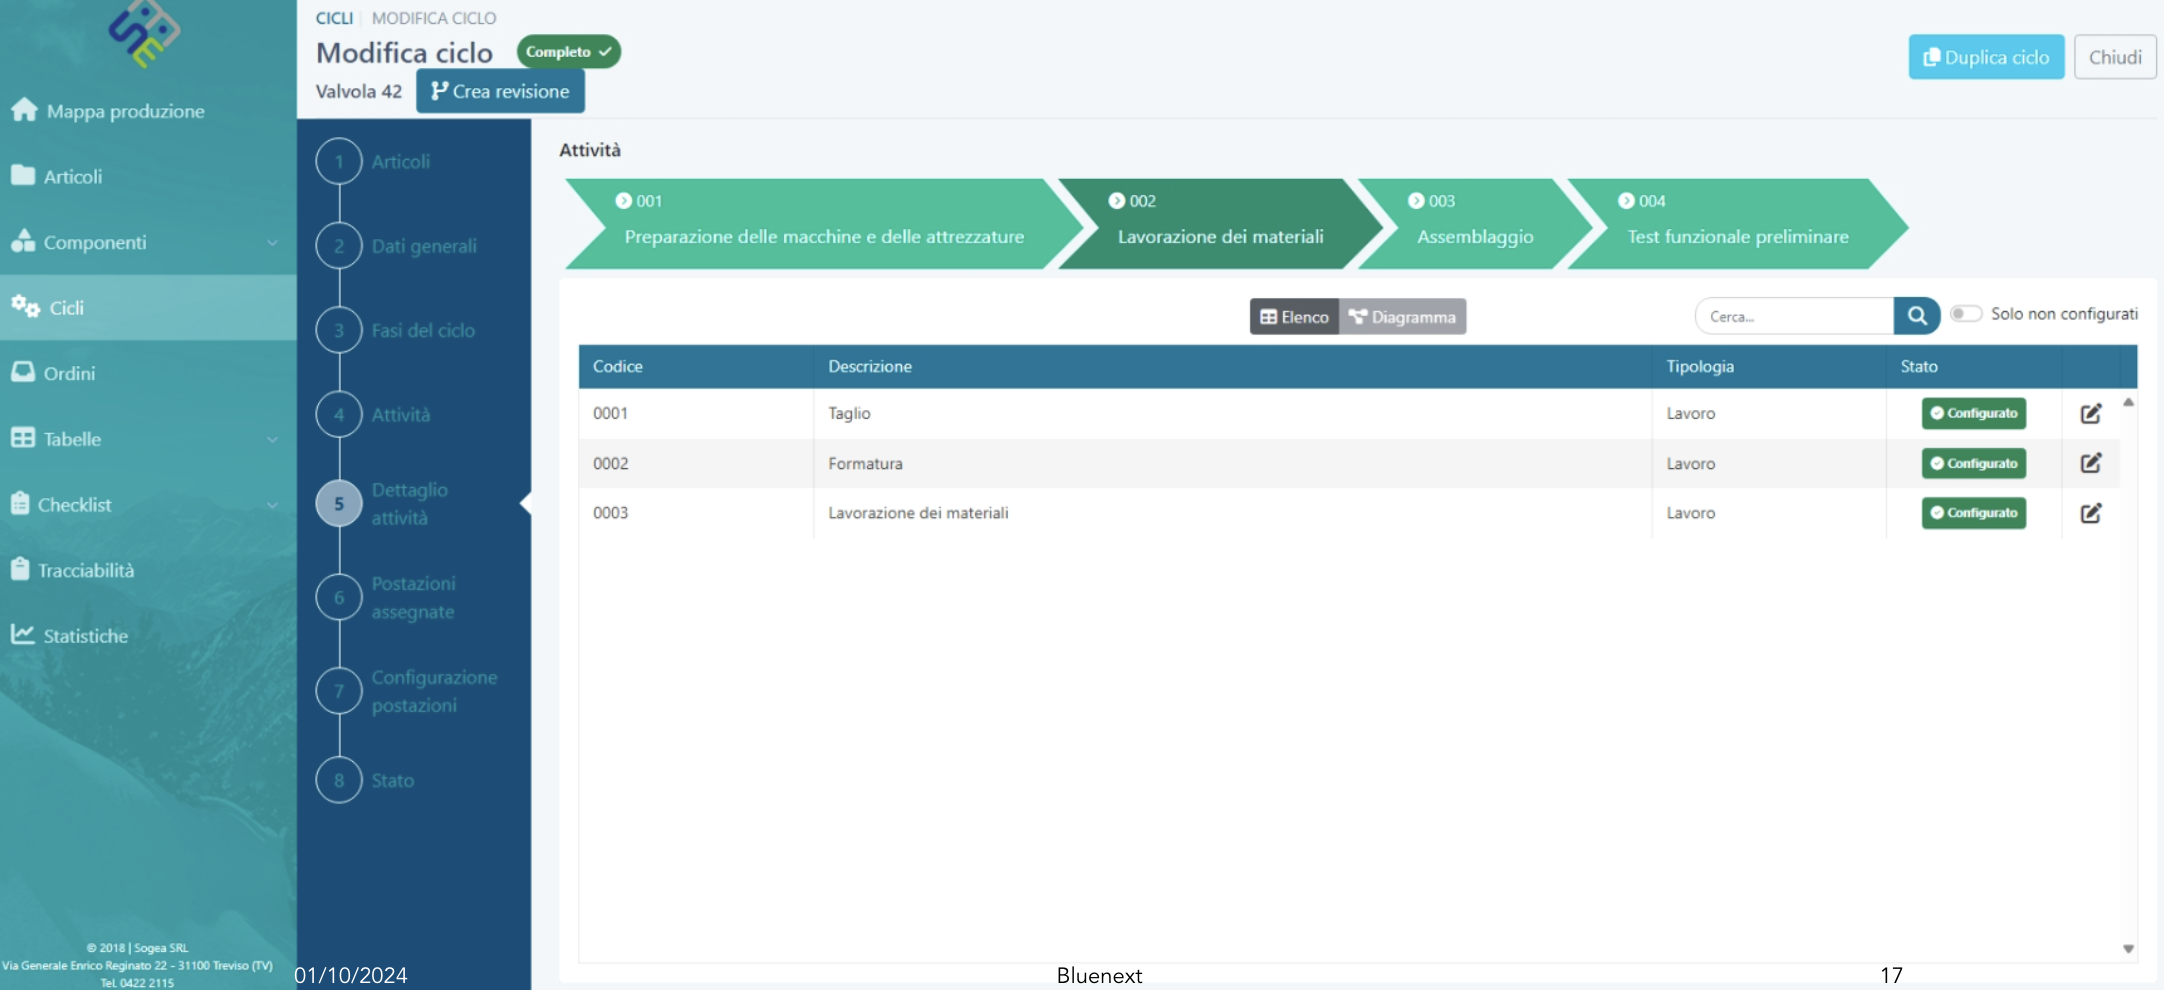
\includegraphics[width=1.0\linewidth]{BCS-Tessi//images/schermata_SAI.png}
            \caption[Schermata del \textit{software} SAI di SogeaSoft S.r.l.]{Schermata del \textit{software} SAI. Fonte: \textit{slide} di presentazione utilizzate durante la fase di formazione}
            \label{fig:screenSAI}
        \end{figure}
        
        \subsection{L'architettura di SAI}
        
            \subsubsection{Il monolite}
            
            Il \textit{software} SAI è caratterizzato da un'architettura monolitica, termine che evoca l'idea di una struttura compatta e unitaria, in cui le varie componenti sono strettamente interconnesse e formano un insieme indivisibile. Nel contesto dell'architettura \textit{software}, tale espressione indica un sistema in cui tutte le funzionalità sono integrate in un'unica unità, costituendo una struttura unificata in cui ciascun componente dipende dagli altri per garantire il corretto funzionamento dell'intero sistema\footnote{O. Al-Debagy and P. Martinek, "A Comparative Review of Microservices and Monolithic Architectures," International Journal of Computer Science and Information Security, vol. 17, no. 3, pp. 123-131, 2019.}.  

            \vspace{0.2 em}
            \noindent Le principali caratteristiche di un'architettura monolitica sono le seguenti:  

            \begin{itemize}
                \item \textbf{integrazione delle funzionalità in un unico blocco applicativo}: tutte le funzionalità sono raccolte in un'unica entità, che viene distribuita come un blocco indivisibile. Questo implica che ogni modifica apportata a una parte del codice può avere ripercussioni su altre parti del sistema, rendendo complessi gli aggiornamenti e la manutenzione. Di conseguenza, con l'evolversi del progetto, l'accumulo di \text{debito tecnico\textsubscript{G}} può far sì che il \textit{software} diventi eccessivamente complesso e difficilmente adattabile a nuove tecnologie\footnote{J. Fritzsch, J. Bogner, A. Zimmermann, and S. Wagner, "From Monolith to Microservices: A Classification of Refactoring Approaches," in Proceedings of the IEEE International Conference on Software Architecture (ICSA), Stuttgart, Germany, 2018.};
                \item  \textbf{scalabilità verticale}: la scalabilità in un sistema monolitico si ottiene potenziando l'intera applicazione per affrontare un aumento del carico di lavoro\ap{3}. Anche qualora solo alcune funzionalità necessitassero di risorse aggiuntive, l'intero sistema deve essere aggiornato, comportando uno spreco di risorse. Non essendo sempre possibile una scalabilità modulare, si tende a duplicare l'intera applicazione per garantire le prestazioni richieste;
                \item \textbf{bassa} \text{\textbf{granularità}\textsubscript{G}}: l'architettura monolitica presenta una scarsa separazione delle funzionalità, che risultano strettamente integrate e difficilmente isolabili\footnote{M. Cojocaru, A. Uta, and A.-M. Oprescu, "MicroValid: A Validation Framework for Automatically Decomposed Microservices," in Proceedings of the 11th IEEE/ACM International Conference on Cloud Computing (CloudCom), December 2019.}. Questo limita significativamente la flessibilità del sistema e ostacola l'integrazione di nuovi moduli o tecnologie senza compromettere la stabilità complessiva; 
                \item \textbf{\textit{database} centralizzato}: ciò implica che tutte le componenti dell'applicazione accedono e manipolano direttamente gli stessi dati. Questo comporta un \textbf{forte accoppiamento \textit{(tightly coupled)}}\footnote{Fonte: https://martinfowler.com/articles/break-monolith-into-microservices.html \textit{(ultima visita 14/03/2025)}} tra i moduli e rende complessi gli aggiornamenti o le modifiche al \textit{database}, poiché qualsiasi cambiamento può avere ripercussioni sull'intero sistema.
            \end{itemize}  

            \vspace{0.2 em}
            \noindent L'architettura monolitica del sistema SAI rappresenta una sfida significativa in termini di manutenibilità e adattabilità alle tecnologie moderne. Tale struttura, caratterizzata da un'elevata interdipendenza tra i componenti, limita la capacità di evoluzione e di risposta ai cambiamenti del contesto operativo. Questa situazione evidenzia la necessità di intraprendere un percorso di migrazione verso un'architettura a microservizi, che consentirebbe di migliorare la modularità del sistema attraverso componenti indipendenti e specializzati. 

            \subsubsection{I microservizi}
            
            Al contrario, un'architettura basata su microservizi presenta caratteristiche distintive che la differenziano in modo significativo da quella monolitica, garantendo maggiore flessibilità e modularità.            
            
            \noindent Riprendendo i punti descritti nella precedente sezione, segue una descrizione delle principali caratteristiche di questa architettura:  

            \begin{itemize}
                \item \textbf{funzionalità distribuite in più \textit{codebase}}: le funzionalità del sistema sono organizzate in servizi separati, ognuno dei quali dispone di una propria \textit{codebase} autonoma\footnote{O. Al-Debagy and P. Martinek, "A Comparative Review of Microservices and Monolithic Architectures," International Journal of Computer Science and Information Security, vol. 17, no. 3, pp. 123-131, 2019.}. I microservizi comunicano tra loro tramite reti, spesso utilizzando API, mantenendo un elevato grado di indipendenza;
                \item \textbf{scalabilità orizzontale}: è possibile aumentare le risorse relative a una singola funzionalità semplicemente aggiungendo istanze del microservizio corrispondente\footnote{Fonte: https://dev.to/somadevtoo/horizontal-scaling-vs-vertical-scaling-in-system-design-3n09 \textit{(ultima visita: 14/03/2024)}}, senza dover stratificare l'intera applicazione. In un contesto di \textit{Domain-Driven Design} (DDD), si parla di \textbf{evoluzione del dominio}, ossia della capacità di migliorare e adattare il sistema in funzione dei cambiamenti del dominio applicativo\footnote{E. Evans, Domain-Driven Design: Tackling Complexity in the Heart of Software, Addison-Wesley, 2003}, evitando di creare monoliti stratificati e complessi da gestire (come ad esempio SAI);
                \item \textbf{alta granularità}: l'architettura a microservizi è caratterizzata da un'elevata granularità\footnote{M. Cojocaru, A. Uta, and A.-M. Oprescu, "MicroValid: A Validation Framework for Automatically Decomposed Microservices," in Proceedings of the 11th IEEE/ACM International Conference on Cloud Computing(CloudCom), December 2019}, in cui ogni servizio è dedicato a una specifica funzionalità e opera in modo autonomo. Questa separazione netta consente di mantenere una chiara distinzione tra le responsabilità dei vari servizi, agevolando la manutenibilità e l'evoluzione del sistema. Il DDD supporta questa fase attraverso la definizione di \textbf{Bounded Contexts} e l'applicazione del principio di \textbf{Separation of Concerns}\ap{9}, che garantiscono una chiara demarcazione tra i diversi ambiti di competenza e funzionalità.  
                \item \textbf{database distribuito}: i microservizi dispongono di database indipendenti\footnote{S. Newman, Monolith to Microservices: Evolutionary Patterns to Transform Your Monolith, O'Reilly Media, 2019.}. Ogni microservizio è responsabile della gestione dei propri dati e, qualora necessiti di informazioni da un altro servizio, effettua una richiesta esplicita tramite meccanismi di comunicazione inter-servizio, spesso implementati tramite \textbf{Domain Events}\ap{9}. Questo approccio riduce il forte accoppiamento (\textbf{\textit{loose coupling}})\footnote{Fonte:https://martinfowler.com/articles/break-monolith-into-microservices.html (ultima visita 14/03/2025)} tra le componenti, garantendo maggiore modularità e resilienza del sistema. 
            \end{itemize}  

            \vspace{0.2 em}
            \noindent Queste caratteristiche rendono l'architettura a microservizi particolarmente adatta a contesti dinamici e complessi, in cui la capacità di adattamento e la modularità rivestono un ruolo fondamentale nel garantire la qualità e la manutenibilità del sistema. Nella pratica applicativa, tuttavia, tali caratteristiche ideali non sempre trovano piena realizzazione. I sistemi reali presentano spesso complessità intrinseche che rendono difficoltosa una netta separazione delle funzionalità, mentre vincoli di natura economica, temporale o tecnica possono limitare la possibilità di effettuare migrazioni complete verso questa architettura. 

            \noindent L'implementazione dei microservizi richiede pertanto un approccio pragmatico che consideri attentamente il contesto specifico, valutando il rapporto costi-benefici delle diverse soluzioni possibili. Questo implica accettare l'inevitabile assenza di soluzioni perfette e adottare strategie incrementali che consentano di bilanciare gli obiettivi architetturali con i vincoli operativi.

            \vspace{0.2 em}
            \noindent L'obiettivo del mio \textit{stage} è quello di fornire una base formale e metodologica al lavoro empirico già avviato da SogeaSoft S.r.l. riguardo alla migrazione verso un'architettura a microservizi, con l'intento di superare i limiti strutturali del sistema attuale e di garantire una maggiore flessibilità e scalabilità in futuro. Una rappresentazione visuale di questa attività è visibile nella Figura \ref{fig:monolith-vs-microservices}.
            
            \begin{figure}[H]
                \centering
                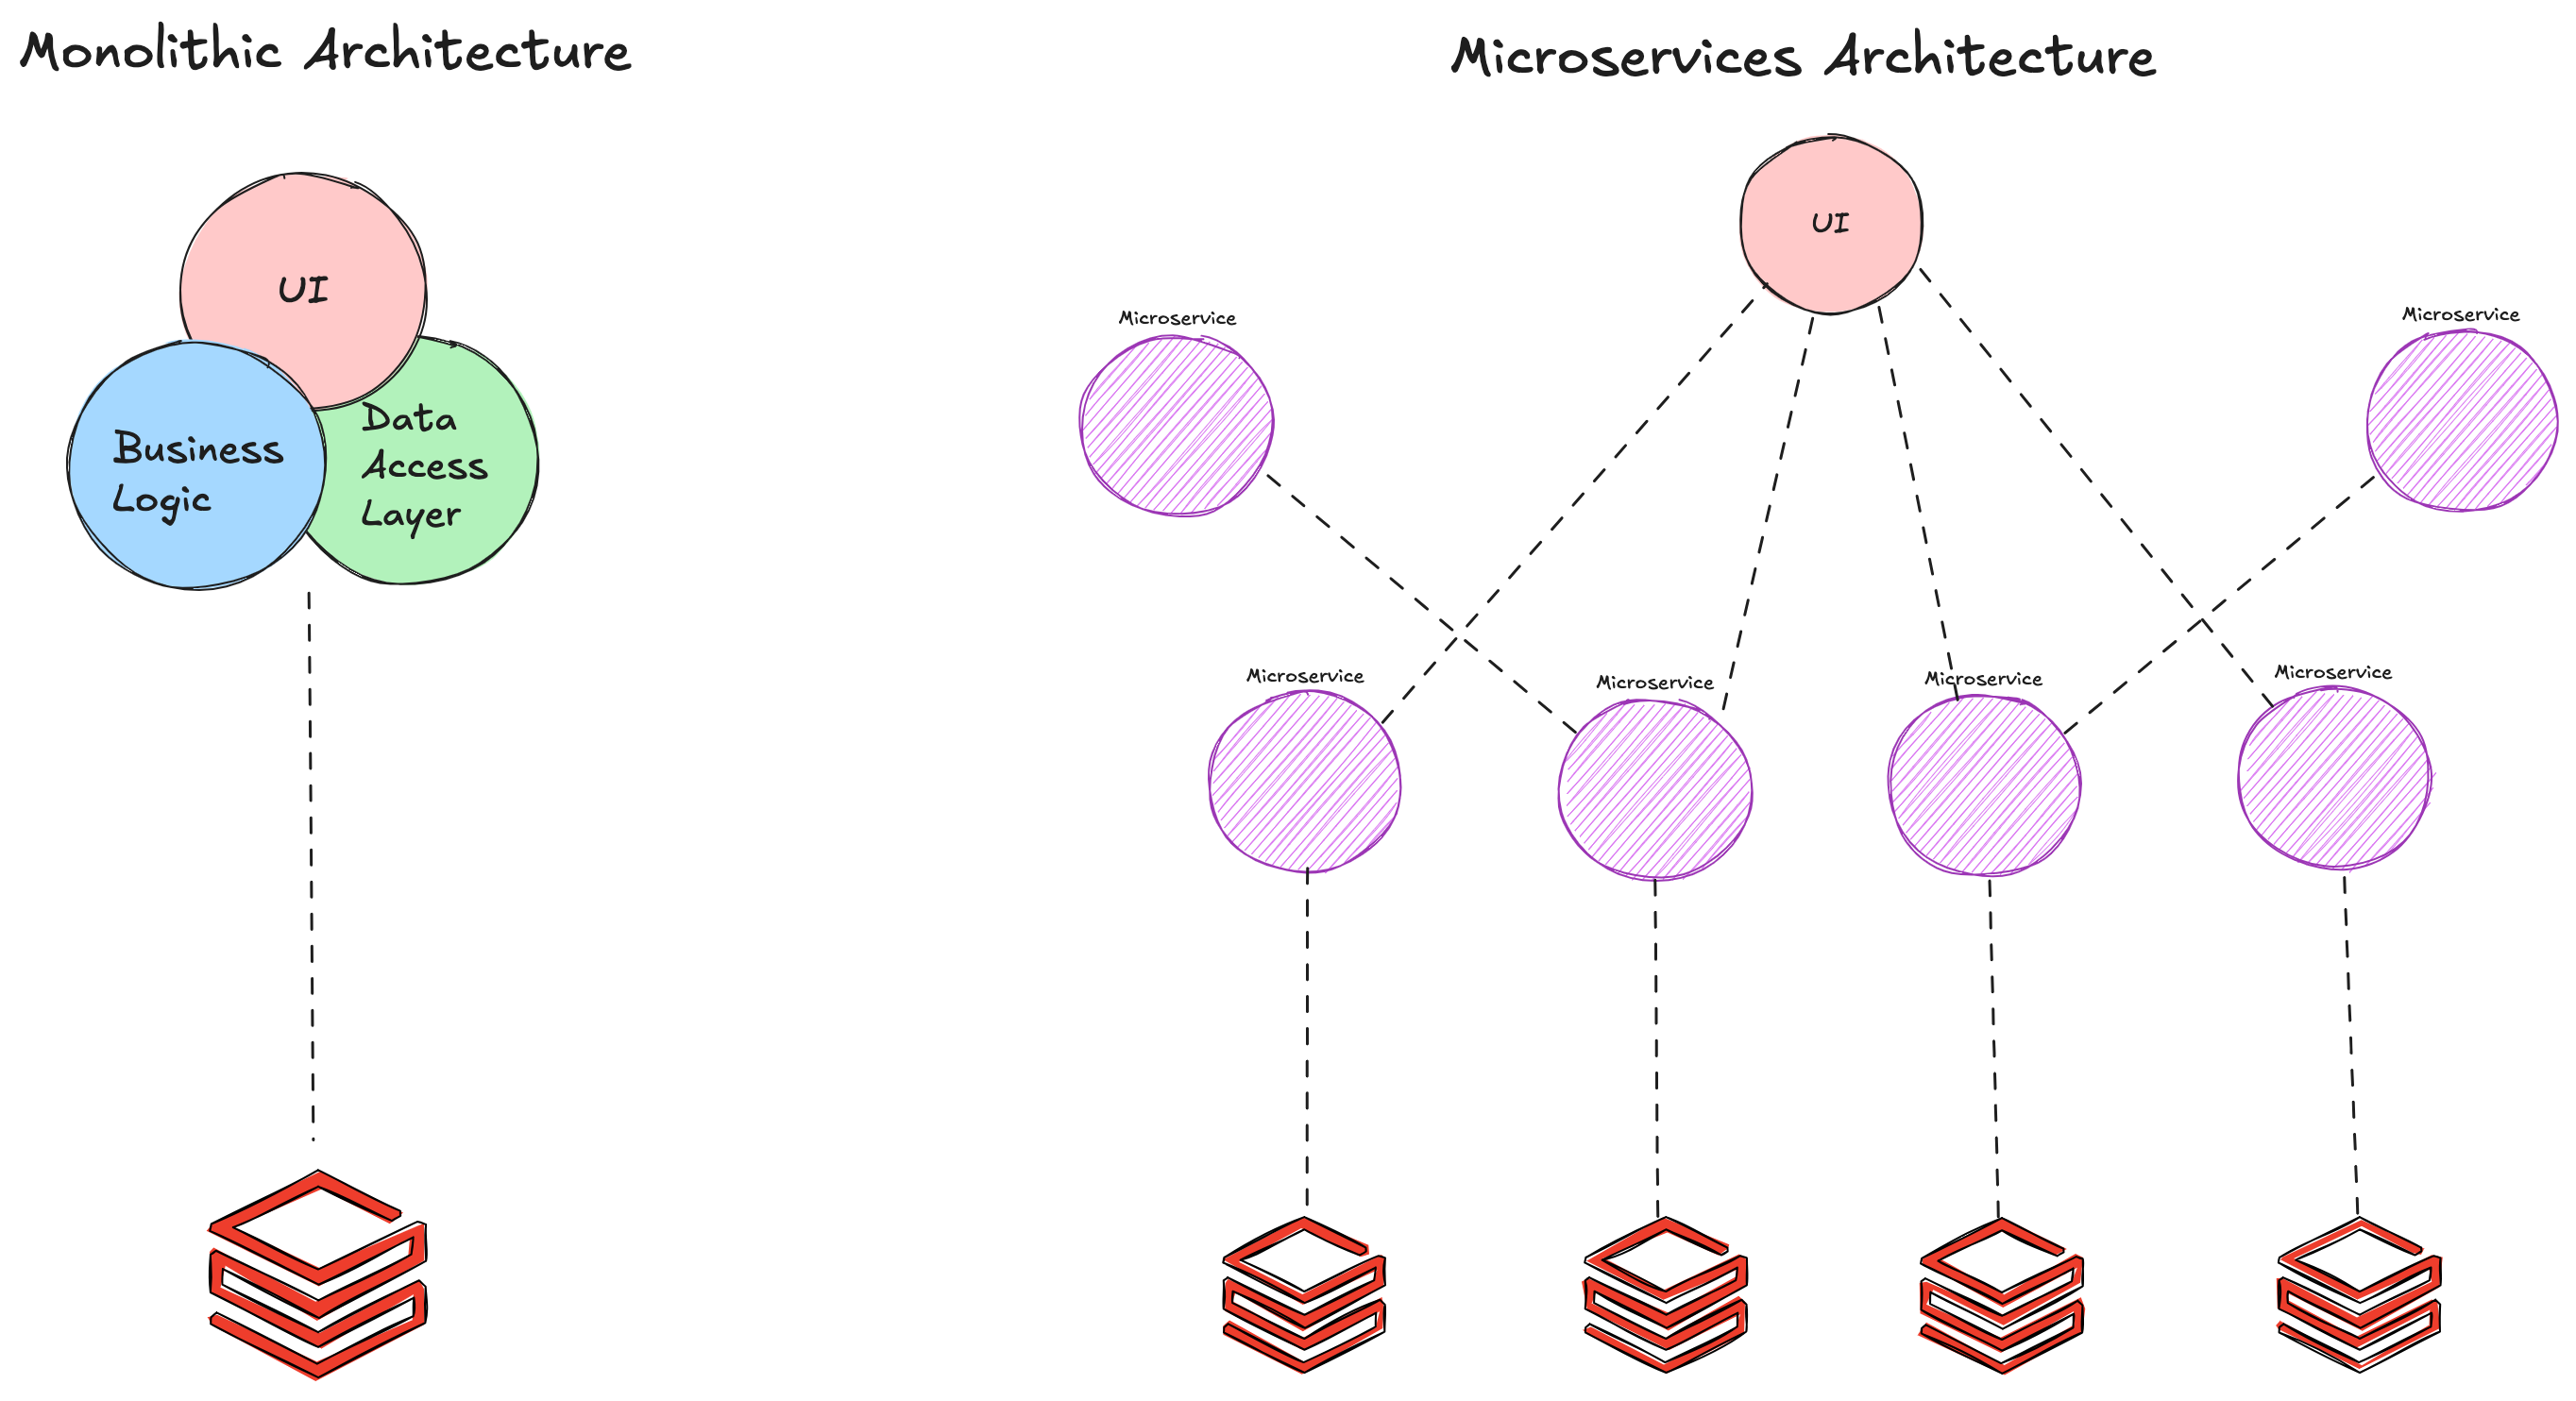
\includegraphics[width=1.0\linewidth]{BCS-Tessi/images/Monolith-Microservices.png}
                \caption[Rappresentazione grafica della suddivisione in microservizi]{Rappresentazione grafica della suddivisione in microservizi}
                \label{fig:monolith-vs-microservices}
            \end{figure}

        \subsection{La migrazione}
        SogeaSoft S.r.l. desidera dunque migrare da un'architettura monolitica a un'architettura a microservizi. Già diverse attività sono state attuate a questo proposito e il mio compito è stato quello di porre una base teorica più solida ed eventualmente confermare o confutare le scelte implementate. Inoltre ho avuto l'occasione di partecipare ai processi decisionali riguardo a particolari casi d'uso nel mio progetto specifico di \textit{stage}. 

        \vspace{0.2 em}
        \noindent Come si può osservare nella Figura \ref{fig:migrazione}, uno degli elementi centrali della migrazione riguarda l'introduzione di una componente denominata MicroService-Middleware, implementata come un \textit{Anti-Corruption $Layer_G$} ($ACL_G$). In ambito architetturale, un ACL è un modello progettuale che funge da interfaccia tra sistemi $legacy_G$ e nuove componenti, prevenendo la propagazione di modelli obsoleti o incoerenti nelle parti più moderne del sistema. Nel contesto di SogeaSoft S.r.l., il MicroService-Middleware si occupa di ricevere le richieste provenienti dall'ERP monolitico e, tramite un \textit{Message $Broker_G$}, instradare tali richieste verso il microservizio appropriato. Il \textit{Message Broker}, infatti, svolge il ruolo di intermediario per lo scambio di messaggi tra componenti \textit{software}, garantendo una comunicazione asincrona ed efficiente tra i vari microservizi.  

        \vspace{0.2 em}
        \noindent Ogni microservizio, una volta attivato, dopo aver effettuato l'autenticazione attraverso l'applicazione nativa di SAI chiamata \textit{Identity Server}, esso esegue la funzione richiesta in modo autonomo e indipendente, restituendo l'esito tramite lo stesso meccanismo di messaggistica. Per rendere accessibili le funzionalità esposte dai microservizi, l'azienda ha implementato una \textit{WebAPI Gateway}, che rappresenta un punto di accesso centralizzato alle API dei vari servizi. La \textit{WebAPI Gateway} consente di aggregare e orchestrare le chiamate ai microservizi, creando un'interfaccia unificata verso l'utente finale.  

        \vspace{0.2 em}
        \noindent Grazie a questa architettura, il sistema è in grado di supportare una \textit{Single Page $Application_G$} (SPA), un tipo di applicazione \textit{web} che carica una singola pagina \textit{web} e aggiorna dinamicamente il contenuto man mano che l'utente interagisce. Questo approccio garantisce un'esperienza utente più fluida e interattiva, riducendo i tempi di caricamento e ottimizzando le \textit{performance} dell'applicazione.  

        \vspace{0.2 em}
        \noindent L'adozione di queste soluzioni riflette la volontà dell'azienda di superare le limitazioni dell'architettura monolitica, garantendo maggiore modularità e adattabilità alle nuove tecnologie, pur mantenendo la continuità dei servizi già in essere.

        \begin{figure}[H]
            \centering
            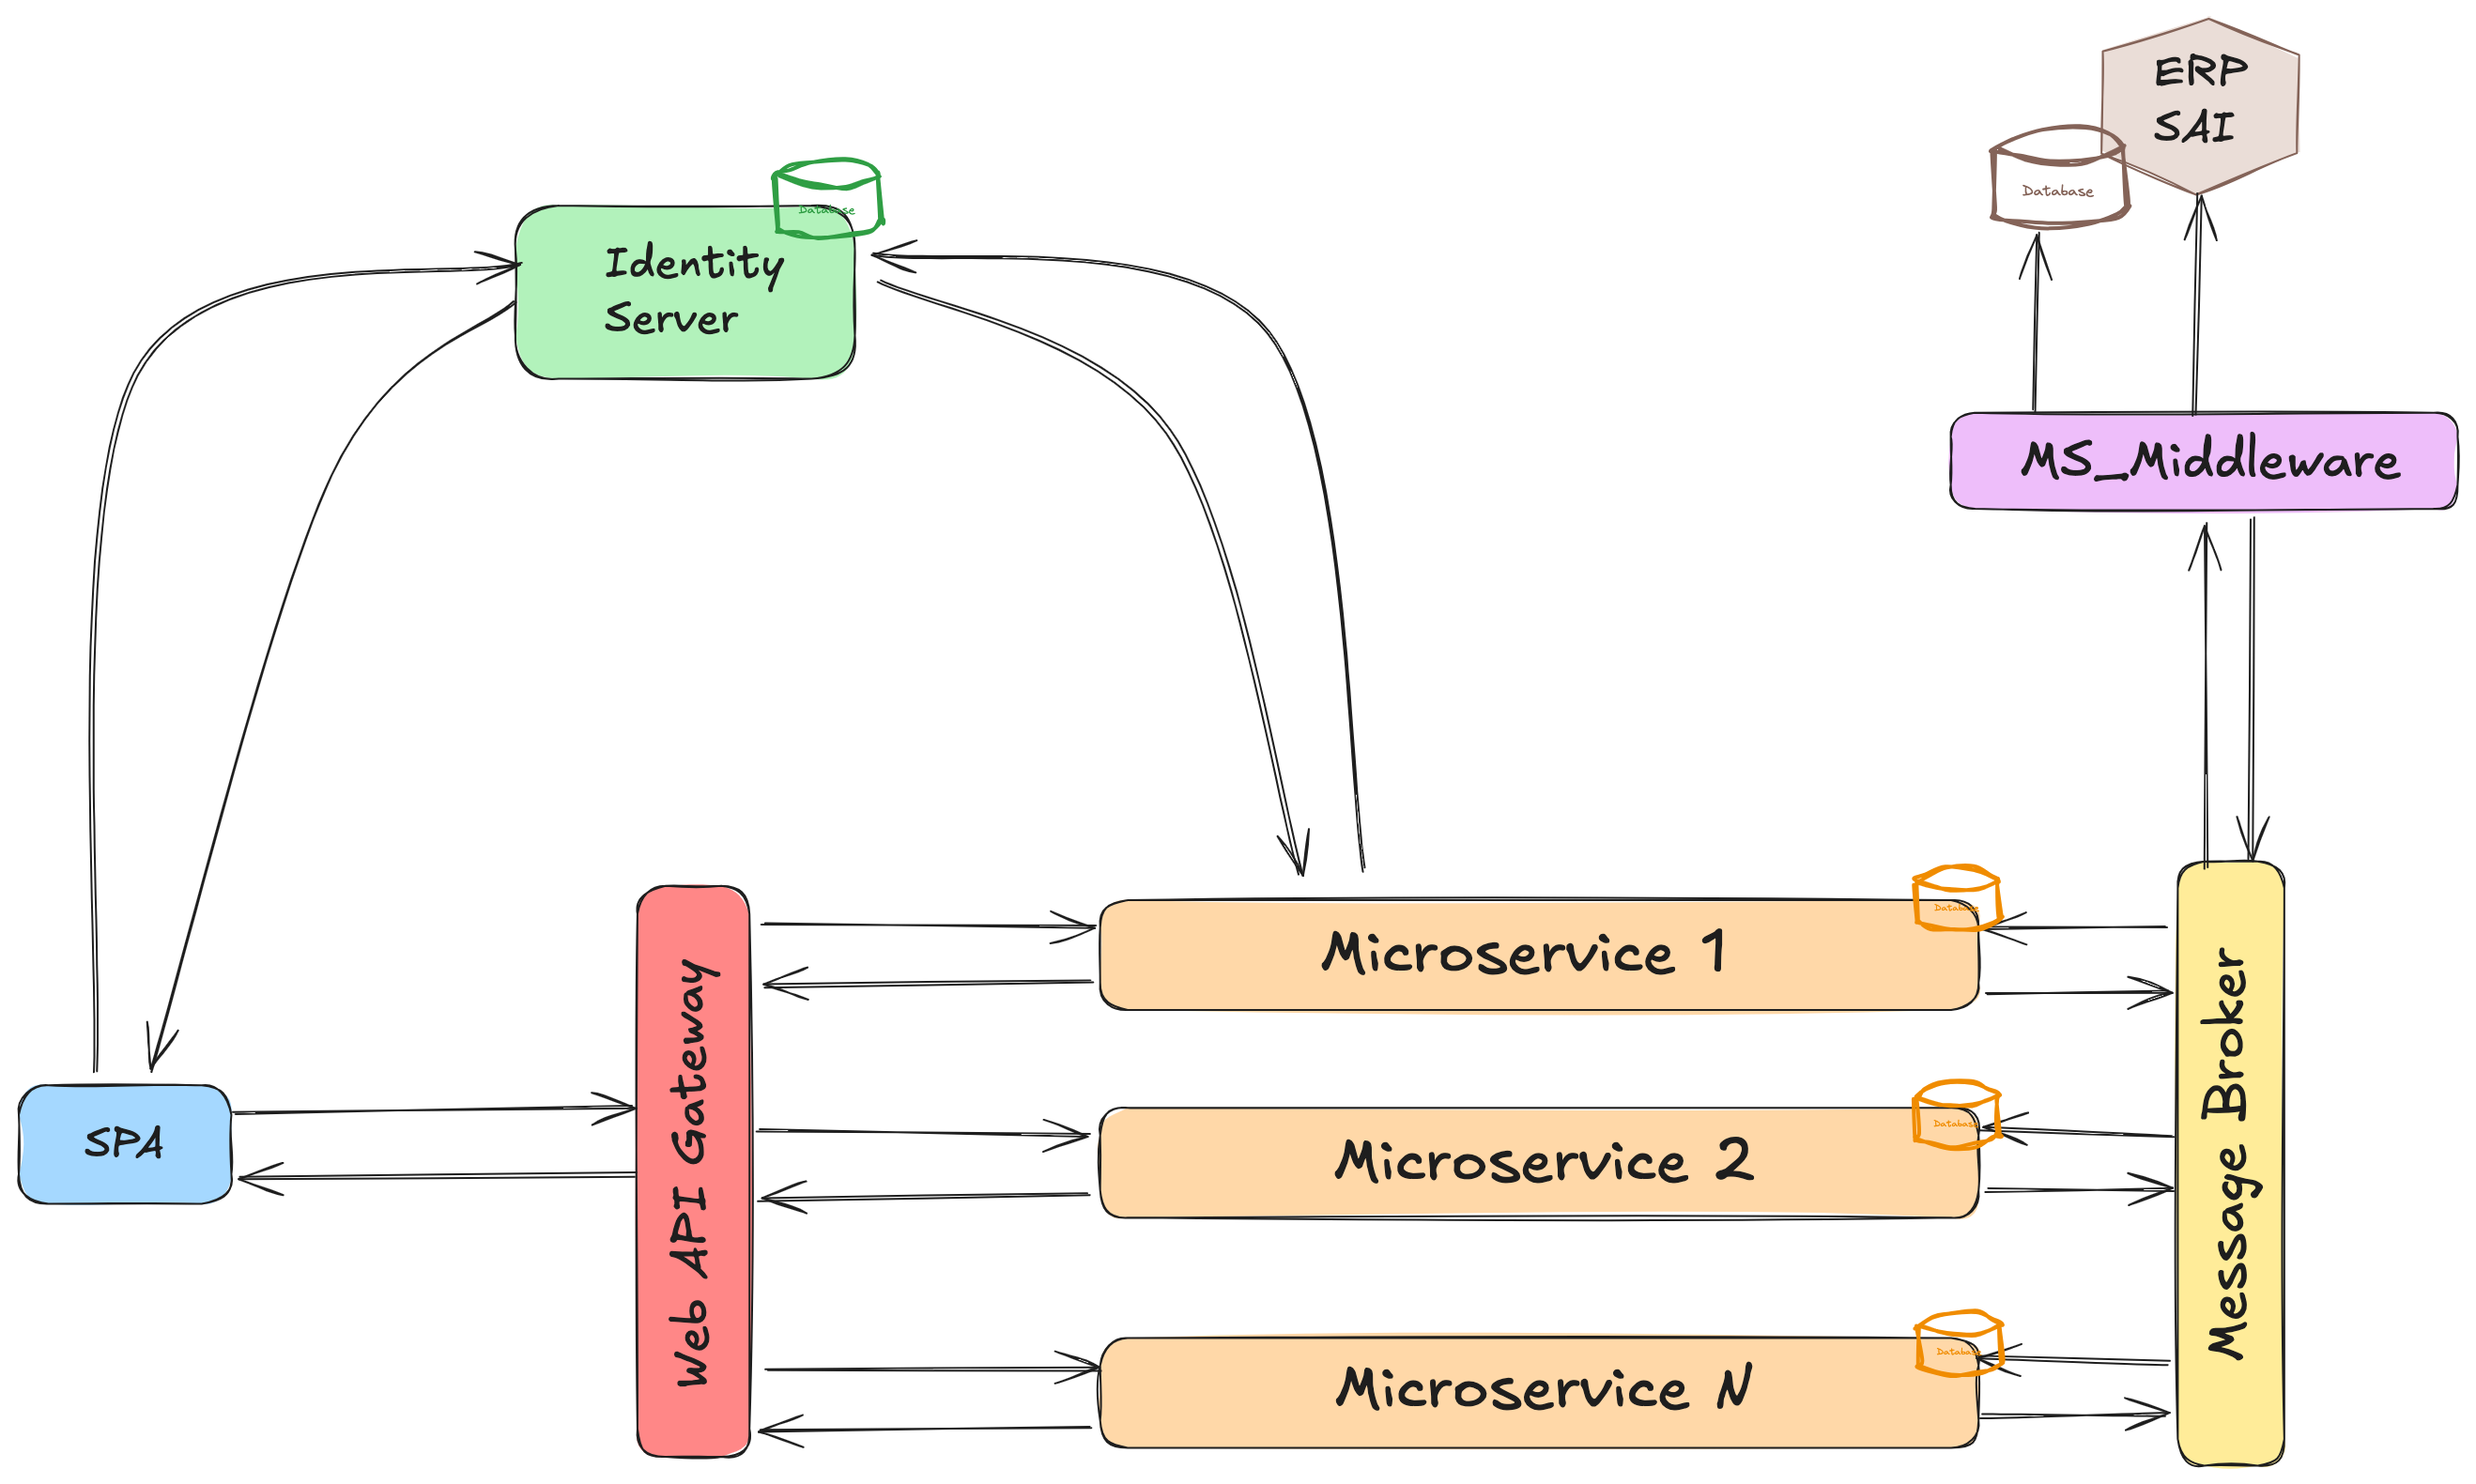
\includegraphics[width=1.0\linewidth]{BCS-Tessi/images/migrazione.png}
            \caption[Piano di migrazione di SogeaSoft S.r.l.]{Piano di migrazione di SogeaSoft S.r.l.. Fonte: informazioni apprese durante il processo di formazione. }
            \label{fig:migrazione}
        \end{figure}
        
    \section{Obiettivi del progetto di \textit{stage}}
        \subsection{Obiettivi aziendali}
        Nel contesto del mio progetto di \textit{stage}, SogeaSoft S.r.l. ha deciso di intraprendere un percorso di approfondimento riguardante la suddivisione del monolite in microservizi. Tale scelta si inserisce nell'ottica di favorire una maggiore modularità e flessibilità del sistema, nonché di facilitare futuri interventi di manutenzione e aggiornamento tecnologico.  

        \vspace{0.2 em}
        \noindent Considerando che l'obiettivo dello \textit{stage} è dimostrare concretamente le competenze acquisite, si è ritenuto opportuno effettuare l'estrazione di un microservizio come risultato tangibile dell'attività svolta. 

        \vspace{0.2 em}
        \noindent A supporto dell'intero progetto, il \textit{tutor} aziendale ha redatto un Piano di lavoro, un documento esaustivo che descrive l'azienda, gli obiettivi progettuali, i vincoli eventualmente presenti, la metodologia adottata e i risultati attesi. Tale documento costituisce un riferimento fondamentale per garantire la coerenza e la chiarezza delle attività intraprese durante lo \textit{stage}. 

        \begin{table}[H]
        \centering
        \renewcommand{\arraystretch}{1.8} % Increase row height by 50%
        \begin{tabular}{|>{\bfseries}c|m{15cm}|} % Use 'm{}' for vertical centering
          \hline
          \multicolumn{2}{|c|}{\textbf{Obiettivi aziendali}} \\ % First row, merged columns
          \hline
          \multicolumn{2}{|c|}{\textbf{Obbligatori}} \\ % Second row, merged columns
          \hline
          \multirow{2}{*}{\vspace*{\fill}OB1\vspace*{\fill}} & Studio della letteratura esistente sulle architetture monolitiche, sulle architetture a microservizi e sui metodi di migrazione \\ 
          \hline
          \multirow{2}{*}{\vspace*{\fill}OB2\vspace*{\fill}} & Documentazione relativa ai requsiti\\ 
          \hline
          \multirow{2}{*}{\vspace*{\fill}OB3\vspace*{\fill}} & Documentazione dei servizi esistenti e delle relazioni tra essi \\ 
          \hline
          \multirow{2}{*}{\vspace*{\fill}OB4\vspace*{\fill}} & Individuazione di un piano indicativo \\ 
          \hline
          \multicolumn{2}{|c|}{\textbf{Desiderabili}} \\ 
          \hline
          \multirow{2}{*}{\vspace*{\fill}DE1\vspace*{\fill}} & Documentazione dei rischi\\ 
          \hline
          \multicolumn{2}{|c|}{\textbf{Facoltativi}} \\ 
          \hline
          \multirow{2}{*}{\vspace*{\fill}FA1\vspace*{\fill}} & Realizzazione del PoC\\ 
          \hline
        \end{tabular}
        \caption[Descrizione degli obiettivi aziendali per il progetto di \textit{stage}]{Descrizione degli obiettivi aziendali per il progetto di \textit{stage}; corrispondono agli obiettivi redatti dal \textit{tutor} aziendale nel Piano di lavoro.}
        \label{tab:obiettivi}
        \end{table}

        \noindent Gli obiettivi aziendali riportati nella Tabella ~\ref{tab:obiettivi} sono classificati secondo la seguente notazione:
        \begin{itemize}
            \item \textbf{Obiettivo obbligatorio (OB)}: rappresentano i requisiti obbligatori, vincolanti, che dovranno necessariamente essere soddisfatti;
            \item \textbf{Obiettivo desiderabile (DE)}: rappresentano i requsiti desiderabili, non vincolanti, ma dal riconoscibile valore aggiunto;
            \item \textbf{Obiettivo facoltativo (FA)}: rappresentano i requisiti facoltativi, rappresentanti di valore aggiunto ma non strettamente competitivo.
        \end{itemize}
        La rappresentazione tabellare utilizza la notazione \textbf{[sigla][identificativo]}, dove la sigla indica la tipologia di obiettivo secondo la classificazione sopra descritta, mentre l'identificativo è un numero progressivo che garantisce l'univocità del requisito in combinazione con la sigla. 

        \subsection{Vincoli}
        
        Per quanto concerne i \textbf{vincoli temporali}, lo \textit{stage} curricolare deve svolgersi nell'arco di un monte ore compreso tra 300 e 320 ore, come previsto dal corso di studi, al fine di garantire un carico di lavoro equivalente a 12 crediti formativi universitari. Nel caso specifico del mio percorso formativo, tali ore sono state distribuite su un periodo di 8 settimane, con un impegno settimanale di 40 ore, articolate dal lunedì al venerdì, dalle ore 8:30 alle ore 17:00.   
        \newpage
        \noindent Per quanto riguarda i \textbf{vincoli tecnologici}, il piano di lavoro ha indicato i seguenti strumenti e metodologie:  
        \begin{itemize}
            \item linguaggio di sviluppo: C\#;
            \item ambiente di sviluppo: Visual Studio, Visual Studio Code;  
            \item metodologia di sviluppo: Scrum (nell'ambito del \textit{framework} \textit{Agile}) e $DevOps_G$, un insieme di pratiche e strumenti che integrano lo sviluppo \textit{software} (Dev) e le operazioni (Ops) volte alla gestione delle infrastrutture tecnologiche. 
        \end{itemize}

        \noindent Tuttavia, nel corso dello \textit{stage} ho avuto l'opportunità di interagire anche con numerose altre tecnologie, che ho approfondito nella Sezione 1.7.

    \section{Metodo di lavoro}
        \subsection{Pianificazione}
        
        Sulla base degli obiettivi di progetto delineati nella Sezione 2.3.1 (Tabella \ref{tab:obiettivi}) e della pianificazione oraria proposta nel Piano di lavoro (Tabella \ref{tab:pianificazione-ore}), insieme al \textit{tutor} aziendale, abbiamo stabilito le principali tappe intermedie (\textit{milestone}) per monitorare il progresso del progetto. La collocazione temporale di queste \textit{milestone} è stata determinata tenendo conto sia delle attività che dipendono strettamente l'una dall'altra, in particolare per quanto riguarda gli aspetti formativi, sia della necessità di produrre risultati tangibili, quali documentazione e codice in modo regolare. Ciò ha permesso al \textit{tutor} di monitorare il progresso del progetto e individuare tempestivamente eventuali rallentamenti.

        \vspace{0.2 em}
        \noindent La definizione dettagliata delle singole attività è avvenuta nel corso delle sessioni di \textit{Sprint planning} con il \textit{Product Owner}. Durante questi incontri, mi venivano assegnate le attività specifiche, venivano chiariti i risultati attesi e venivano fissati appuntamenti per valutare il grado di avanzamento, fornire supporto in caso di difficoltà o testare i risultati raggiunti. 

        \renewcommand{\arraystretch}{2} % Increase row height globally
        \setlength{\tabcolsep}{9pt} % Increase horizontal padding in cells
        
        \begin{longtable}{|>{\bfseries}c|m{13cm}|}
          \hline
          \multirow{2}{*}{\makecell{\vspace*{5mm}Durata in ore\vspace*{5mm}}} & \textbf{Descrizione attività} \\ 
          \hline
          \endfirsthead % Header for the first page
          \hline
          \multirow{2}{*}{\makecell{\vspace*{5mm}Durata in ore\vspace*{5mm}}} & \textbf{Descrizione attività} \\ 
          \hline
          \endhead % Header for subsequent pages
          \hline
          \multicolumn{2}{|r|}{{Continua nella pagina successiva}} \\ 
          \endfoot % Footer for all pages except the last
          
          \endlastfoot
        
          \multirow{2}{*}{\makecell{\vspace*{5mm}16\vspace*{5mm}}} & Conoscenza ambiente di lavoro e contesto\\ 
          \hline
          \multirow{2}{*}{\makecell{\vspace*{5mm}32\vspace*{5mm}}} & Studio della letteratura esistente sulle architetture monolitiche, sulle architetture a microservizi e sui metodi di migrazione\\ 
          \hline
          \multirow{2}{*}{\makecell{\vspace*{5mm}24\vspace*{5mm}}} & Analisi dell'applicazione esistente per identificare i servizi e le funzionalità da suddividere in microservizi\\ 
          \hline
          \multirow{2}{*}{\makecell{\vspace*{5mm}16\vspace*{5mm}}} & Stesura della documentazione relativa ai requisiti\\
          \hline
          \multirow{2}{*}{\makecell{\vspace*{5mm}24\vspace*{5mm}}} & Studio dell'architettura a microservizi già esistente e analisi dei possibili miglioramenti per facilitarne la migrazione\\
          \hline
          \multirow{2}{*}{\makecell{\vspace*{5mm}32\vspace*{5mm}}} & Identificazione dei servizi monolitici da decomporre e delle relazioni tra essi.\\
          \hline
          \multirow{2}{*}{\makecell{\vspace*{5mm}24\vspace*{5mm}}} & Documentazione dei servizi esistenti e delle relazioni tra essi e del piano\\
          \hline
          \multirow{2}{*}{\makecell{\vspace*{5mm}16\vspace*{5mm}}} & Identificazione dei potenziali rischi e delle sfide associate alla migrazione\\
          \hline
          \multirow{2}{*}{\makecell{\vspace*{5mm}24\vspace*{5mm}}} & Inizio dello sviluppo di un Proof of Concept\\
          \hline
          \multirow{2}{*}{\makecell{\vspace*{5mm}16\vspace*{5mm}}} & Documentazione dei rischi\\
          \hline
          \multirow{2}{*}{\makecell{\vspace*{5mm}8\vspace*{5mm}}} & Individuazione di un piano indicativo di migrazione\\
          \hline
          \multirow{2}{*}{\makecell{\vspace*{5mm}24\vspace*{5mm}}} & Proseguimento del Proof of Concept\\
          \hline
          \multirow{2}{*}{\makecell{\vspace*{5mm}16\vspace*{5mm}}} & Valutazione teorica dell'architettura\\
          \hline
          \multirow{2}{*}{\makecell{\vspace*{5mm}32\vspace*{5mm}}} & Revisione della documentazione e del Proof of Concept\\
          \hline
          \multicolumn{2}{|c|}{\textbf{304 ore totali}} \\ % Last row, merged columns
          \hline
          \caption{Ripartizione delle ore in base alle attività} % Caption after the last row
          \label{tab:pianificazione-ore}
        \end{longtable}


        
        \subsection{Modello di sviluppo}
        SogeaSoft S.r.l. adotta un modello di sviluppo \textit{Agile} basato su Scrum, come approfondito nella Sezione 1.4. Tuttavia, durante il mio stage, non ho partecipato a tutte le cerimonie previste dal \textit{framework} Scrum. In particolare, sebbene il \textit{Daily Scrum meeting} si svolgesse quotidianamente con il mio \textit{tutor} (che si alternava al \textit{Product Owner}, in base alla disponibilità e alle necessità di ciascuno), il mio coinvolgimento nelle altre cerimonie è stato limitato. Infatti, ho partecipato esclusivamente allo \textit{Sprint planning} e alla \textit{Sprint review}, che non avevano una durata fissa, ma variavano a seconda dei \textit{task} assegnati e della disponibilità del \textit{Product Owner}. Nel complesso, il mio lavoro è stato principalmente solitario, con sviluppo individuale e il supporto del \textit{tutor} limitato a momenti specifici. Uno schema utile per visualizzare il processo che ha caratterizzato le attività di sviluppo durante il mio \textit{stage} è visibile in Figura \ref{fig:Sprint-effettivi}.

        \begin{figure}[H]
            \centering
            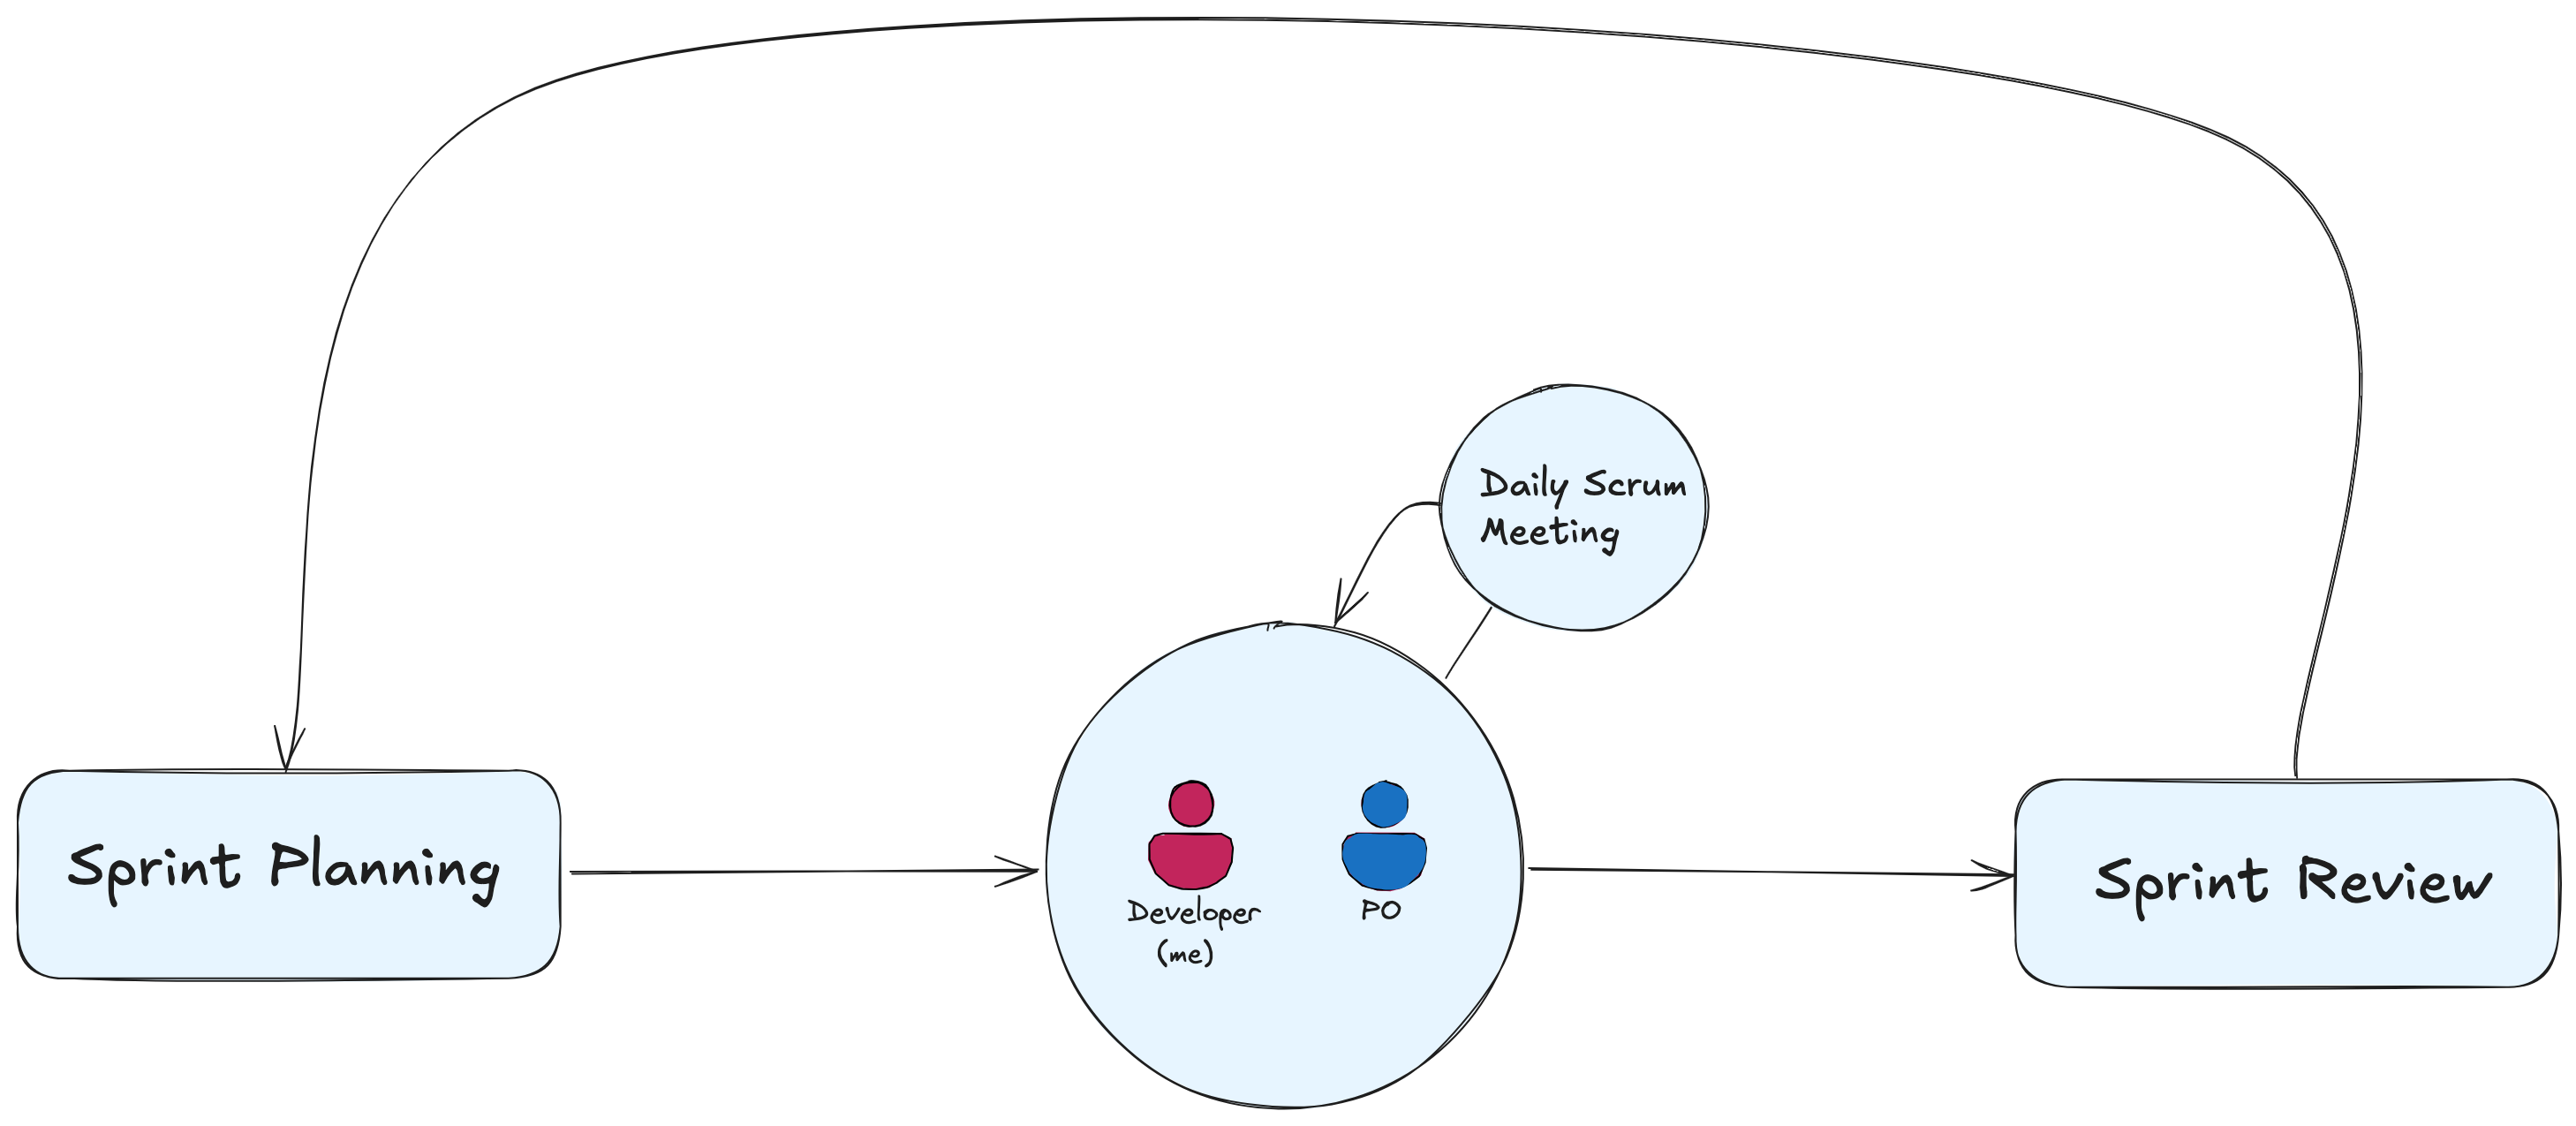
\includegraphics[width=0.7\linewidth]{BCS-Tessi/images/Sprint_true.png}
            \caption[Rappresentazione dell'attività di sviluppo effettiva secondo \textit{Agile} (Scrum)]{Rappresentazione grafica dell'attività di sviluppo effettiva che ha caratterizzato il mio \textit{stage} secondo \textit{Agile}, nel contesto Scrum.}
            \label{fig:Sprint-effettivi}
        \end{figure}
        
        \subsection{Strumenti}
        Gli strumenti utilizzati durante il mio \textit{stage}, oltre alle tecnologie approfondite nella Sezione 1.7, sono stati diversificati e funzionali a diversi aspetti del lavoro. In primo luogo, ho impiegato la documentazione che redigevo progressivamente, utilizzando la \textit{Wiki} di Azure come base di lavoro. Inoltre, per facilitare la gestione delle attività quotidiane e il processo di redazione della tesi, ho creato dei documenti personali in cui annotavo le cose da fare e le note importanti. 

        \vspace{0.2 em}
        \noindent Ogni sessione di \textit{Sprint planning} è stata accompagnata dalla definizione dettagliata dei \textit{task} da parte del \textit{Product Owner}, al fine di evitare ambiguità nell'interpretazione delle attività. Questi \textit{task} sono stati organizzati e conservati in una cartella Drive, dove ho anche archiviato libri, articoli e altre fonti utili trovate durante il progetto. 

        \vspace{0.2 em}
        \noindent Poiché le pianificazioni erano gestite in modo intuitivo, non è stato necessario un ricorso frequente al calendario, in quanto il \textit{Product Owner} mi comunicava direttamente le date degli incontri successivi. Un ulteriore strumento di monitoraggio utile è stato il \textit{report} settimanale, che inviavo al mio \textit{tutor} interno. Questi \textit{report} mi hanno permesso di tracciare lo stato di avanzamento del progetto, identificare eventuali rallentamenti o problematiche, e di valutare se fosse opportuno rivedere le priorità tra le attività in corso.
        
        \subsection{Revisioni di progresso}

        Durante l'intero periodo di \textit{stage}, le interazioni con il \textit{tutor} aziendale sono state caratterizzate da una costante frequenza e prossimità. La vicinanza fisica delle postazioni lavorative ha notevolmente facilitato le opportunità di confronto professionale, contribuendo a mitigare la naturale difficoltà nell'avanzare richieste di supporto. Ciononostante, uno dei primi \textit{feedback} che ho ricevuto ha riguardato la necessità di incrementare la frequenza delle richieste di assistenza, evitando un'eccessiva ostinazione nella ricerca autonoma di soluzioni, e di migliorare la comunicazione complessiva, sia in merito ai progressi conseguiti che alle criticità riscontrate.

        \vspace{0.2 em}
        \noindent In aggiunta agli incontri giornalieri individuali (\textit{Daily meeting}), che si svolgevano successivamente alle riunioni del \textit{tutor} relative ai suoi progetti, ho sistematicamente beneficiato dell'opportunità di comunicare l'avanzamento delle attività o le problematiche incontrate, senza la necessità di attendere la successiva sessione programmata.

        \vspace{0.2 em}
        \noindent Le valutazioni formali dei progressi, condotte con l'altro \textit{Product Owner}, avvenivano nell'ambito degli \textit{Sprint Review}, durante i quali questo verificava l'efficacia funzionale del lavoro svolto. In due circostanze distinte ho presentato il prototipo sviluppato all'intero \textit{team} di sviluppo, considerata l'immediata applicabilità dello stesso. Tali presentazioni hanno costituito di fatto l'illustrazione del prodotto finale. La seconda occasione ha riguardato lo sviluppo di una dimostrazione funzionale (PoC) relativa a una funzionalità di particolare interesse: la sincronizzazione dei dati in tempo reale.
        
    \section{Motivazioni della scelta}
    La selezione dell'opportunità di \textit{stage} è stata guidata da una riflessione evolutiva sulla natura e sugli obiettivi formativi di tale esperienza. Inizialmente, consideravo lo \textit{stage} prevalentemente come un'occasione di applicazione pratica delle conoscenze teoriche acquisite durante il percorso accademico. Tuttavia, la partecipazione all'evento STAGE-IT, tenutosi a Padova nell'aprile 2024, ha determinato un ampliamento di tale prospettiva, conducendomi a pensare l'esperienza di \textit{stage} anche come un'opportunità di sviluppo professionale e personale nonché di confronto con sfide innovative.

    \vspace{0.2 em}
    \noindent L'architettura a microservizi, approfondita teoricamente durante il corso di Ingegneria del \textit{Software}, aveva suscitato in me un particolare interesse, che non aveva trovato adeguate opportunità di esplorazione pratica nell'ambito dei progetti didattici. L'individuazione di una proposta di \textit{stage} focalizzata su tale paradigma architetturale ha rappresentato pertanto un'opportunità particolarmente rilevante per il mio percorso formativo. La reciproca soddisfazione nella selezione è stata ulteriormente confermata dall'interesse manifestato dall'azienda per la mia candidatura, considerata la limitata attrattività del progetto tra gli altri studenti.

    \vspace{0.2 em}
    \noindent Sottolineo che la decisione è stata principalmente determinata dall'interesse per la tematica progettuale, piuttosto che da una preesistente conoscenza o affinità con l'azienda ospitante. La natura manifatturiera di SogeaSoft S.r.l. non ha costituito un elemento determinante nella selezione, poiché un'attività di tipo artigianale sarebbe risultata maggiormente in linea con i miei ideali, in contrapposizione all'ottimizzazione della produzione industriale su larga scala. Inoltre, è emerso come l'interesse principale dell'azienda sia di natura economica, senza una significativa considerazione per la sostenibilità o l'impatto ambientale. Sebbene sia vero che il miglioramento dell'efficienza possa talvolta contribuire alla riduzione degli sprechi, qualora ciò sia avvenuto si tratta di un esito accidentale piuttosto che intenzionale.

    
        \subsection{Obiettivi e aspettative personali}
        \noindent La scelta dello \textit{stage} è stata dunque guidata da motivazioni personali, in particolare dalla curiosità verso l'argomento specifico dei microservizi.

        \vspace{0.2 em}
        \noindent L'esperienza precedente con il progetto di Ingegneria del \textit{Software} mi ha permesso di identificare alcuni aspetti personali da migliorare e argomenti tecnici da approfondire. Tra questi, il mio interesse per i microservizi, che ho descritto in dettaglio nella sezione 2.5, e per le API come metodi di comunicazione tra microservizi. Durante il progetto universitario, non ho avuto l'opportunità di esplorare adeguatamente questi temi, sia per una non ottimale organizzazione del gruppo di lavoro, sia per una distribuzione inefficace delle attività. Mi sono ritrovata infatti a dedicare tempo ad attività poco significative (\textit{shallow work}) a discapito di altre più formative, tra cui l'approfondimento di queste tecnologie che producono reale valore, che rappresentano un esempio di attività di \textit{deep work}\footnote{C. Newport, Deep Work: Rules for Focused Success in a Distracted World, Grand Central Publishing, 2016}.

        \vspace{0.2 em}
        \noindent Questa esperienza mi ha fatto comprendere come la scarsa fiducia nelle mie capacità e la difficoltà nel comunicare apertamente (sia le difficoltà che i progressi) mi abbiano portato ad una situazione in cui le decisioni venivano prese da altri per me. Questi aspetti sono diventati obiettivi di miglioramento personale, per i quali lo \textit{stage} ha rappresentato un'importante opportunità di crescita.

        \vspace{0.2 em}
        \noindent Sebbene ritenessi di aver già fatto progressi nelle mie capacità comunicative, i \textit{feedback} ricevuti dal \textit{tutor} aziendale mi hanno fatto comprendere che ero solo all'inizio di questo percorso di sviluppo personale.

        \vspace{0.2 em}
        \noindent Analogamente, sempre l'esperienza del corso di Ingegneria del \textit{Software} mi ha insegnato l'importanza di accettare l'assenza di soluzioni perfette nello sviluppo \textit{software} e di comprendere la naturalezza della curva di apprendimento. Durante lo \textit{stage}, ho voluto lavorare sulla capacità di non pretendere risultati perfetti fin da subito, accettando che il processo di apprendimento implica necessariamente la possibilità di non conoscere tutto e di commettere errori come parte integrante della crescita professionale.

        \begin{table}[H]
        \centering
        \renewcommand{\arraystretch}{1.8} % Increase row height by 50%
        \begin{tabular}{|>{\bfseries}c|m{15cm}|} % Use 'm{}' for vertical centering
          \hline
          \multicolumn{2}{|c|}{\textbf{Obiettivi personali}} \\ % First row, merged columns
          \hline
          \multirow{2}{*}{\vspace*{\fill}P1\vspace*{\fill}} & Sviluppare maggiore fiducia nelle mie capacità di \textit{problem solving} e ampliare il repertorio di approcci risolutivi\\ 
          \hline
          \multirow{2}{*}{\vspace*{\fill}P2\vspace*{\fill}} & Approfondire la conoscenza teorica e pratica delle architetture a microservizi, con particolare attenzione ai meccanismi di comunicazione tra servizi\\ 
          \hline
          \multirow{2}{*}{\vspace*{\fill}P3\vspace*{\fill}} & Acquisire la capacità di valutare criticamente le soluzioni tecniche, considerando i compromessi necessari in contesti \textbf{reali} piuttosto che perseguire soluzioni teoricamente perfette\\ 
          \hline
          \multirow{2}{*}{\vspace*{\fill}P4\vspace*{\fill}} & Consolidare la comprensione dei principi di progettazione delle API tra microservizi e delle relative \textit{best practices} implementative\\ 
          \hline
          \multirow{2}{*}{\vspace*{\fill}P5\vspace*{\fill}} & Migliorare nelle competenze di comunicazione professionale, con particolare riferimento alla presentazione tecnica dei risultati durante gli \textit{Sprint review}\\ 
          \hline
          \multirow{2}{*}{\vspace*{\fill}P6\vspace*{\fill}} & Migliorare le capacità di comunicazione interpersonale in ambito lavorativo, sia nella richiesta di supporto che nella condivisione dei progressi conseguiti\\ 
          \hline
          \multirow{2}{*}{\vspace*{\fill}P7\vspace*{\fill}} & Sviluppare una maggiore consapevolezza del processo di apprendimento professionale, accettando la naturale curva di apprendimento e la progressiva acquisizione di competenze\\ 
          \hline
          \multirow{2}{*}{\vspace*{\fill}P8\vspace*{\fill}} & Ottimizzare la gestione del tempo lavorativo attraverso un approccio più strutturato e consapevole, privilegiando periodi prolungati di \textit{deep work}, ossia concentrazione profonda\\ 
          \hline
        \end{tabular}
        \caption[Tabella degli obiettivi personali]{Tabella degli obiettivi personali nel contesto dello svolgimento dello \textit{stage}}
        \label{tab:obiettivi-personali}
        \end{table}